
\documentclass[aps,twocolumn,secnumarabic,nobalancelastpage,amsmath,amssymb,
nofootinbib]{revtex4}
%\usepackage[left=0.6in,top=0.5in,right=0.85in,bottom=0.6in]{geometry}
% nofootinbib is another document class option that allows you to put
% footnotes on the page where they occur rather than at the end of the
% paper.  This makes for easier reading!

% secnumarabic is a particularly nice way of identifying sections by
% number to aid electronic review and commentary.

% amsmath and amssymb are necessary for the subequations environment
% among others

%\usepackage{graphics}      % standard graphics specifications
%\usepackage{graphicx}      % alternative graphics specifications
\usepackage{longtable}     % helps with long table options
\usepackage{url}           % for on-line citations
\usepackage{bm}            % special 'bold-math' package
\usepackage[pdftex]{graphicx}
\usepackage[pdftex,colorlinks=true,pdftitle ={ASTR510 Final Paper},pdfauthor = {Daniel George} ]{hyperref}  %Hyperlinking
%\hypersetup{colorlinks,	citecolor=Green,filecolor=Yellow,	linkcolor=Red,	urlcolor=Blue,	pdftex}

\begin{document}
	\title{Simulations of Binary Black Hole Mergers with the Einstein Toolkit}
	\author         {Daniel George}
	\email          {dgeorge5@illinois.edu}
	%\homepage       {http://home.iitb.ac.in/~dan7geo}
	%\affiliation    {Department of Physics}
	\affiliation    {University of Illinois at Urbana-Champaign}
	\date{\today}
	
	\begin{abstract}
	In this paper, I use the Einstein toolkit to perform a fully accurate 3-dimensional numerical relativity simulation of the merger of a binary black hole system with zero spins on a quasi-circular orbit with initial parameters tuned to be identical to GW150914 (the first event detected by LIGO \cite{gw1}). The gravitational waves emitted during the inspiral, merger, and ringdown stages have been extracted and analyzed here. The parameter file and open-source code used to produce this simulation have been made freely available for public use. Scope for extending the simulation to a wider range of parameter values is discussed.
	\end{abstract}
	
	\maketitle
	%%%%%%%%%%%%%%%%%%%%%%%%%%%%%%%%%%%%%%%%%%%%%%%%%%%%%%
	

	\section{Introduction}
	On September 14, 2015, the Advanced Laser-Interferometer Gravitational Wave Observatory (LIGO) detected, for the very first time, gravitational waves (GWs) emitted during the coalescence of two black holes (BHs), shown in figure \ref{ligo}, thus confirming the existence of both gravitational waves and black holes, while paving the way to a new era of gravitational wave astronomy \cite{gw1}. Despite LIGO already being the most precise measurement device ever made, its sensitivity is expected to increase three-fold in the following years, increasing it's observable volume by a factor of 27. Therefore, we will soon have access to a huge influx of gravitational wave data. In the near future, the range of measurable frequencies and the directional sensitivity will be further amplified with the aid of other detectors across the world including VIRGO in Europe, KAGRA in Japan, LIGO in India, NANOGrav (which uses Pulsar Timing Arrays to detect GWs in the nanohertz regime \cite{nano}) and eLISA (the Evolved Laser Interferometer Space Antennae).  The importance of studying binary BHs, the need for gravitational waveforms, and the role of numerical relativity is discussed in the following subsections.

	\begin{figure}[]
		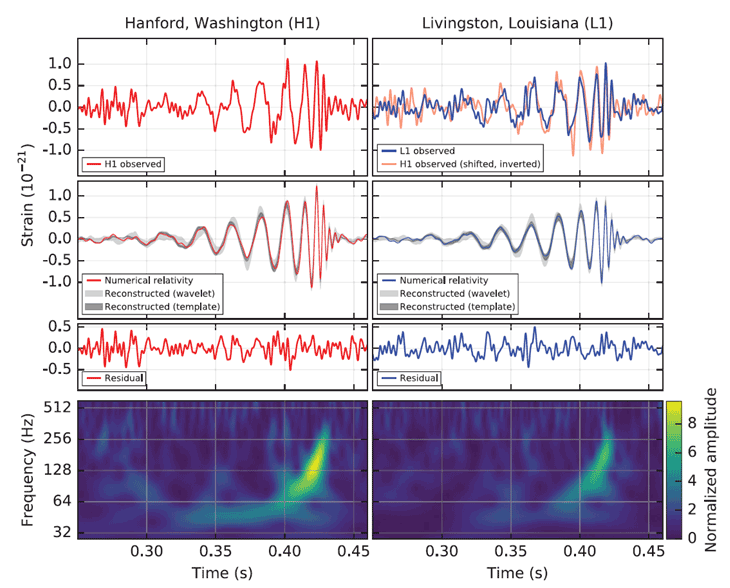
\includegraphics[width=\linewidth]{ligo.png}
		\caption{The first detection by LIGO, named GW150914. \cite{gw1}}
		\label{ligo}
	\end{figure}

	\subsection{Importance of BBH Mergers}
	The importance of binary black hole (BBH) mergers cannot be overstated. They are without doubt the brightest source of gravitational waves in the universe, as far as we know, which explains why all the detections by LIGO until now have been BBH mergers, even though the rate of neutron star mergers are estimated to be higher \cite{LP}. In most cases, we expect no electromagnetic radiation to accompany these events since most of the gas and dust surrounding these black holes are swept away long before they coalesce. In addition, charged black holes, while theoretically allowed, should not exist in nature as they will be instantaneously neutralized by surrounding matter. Therefore, gravitational fields are the only effects involved in these mergers and up to 10\% of the total mass of the system can be converted to pure GW radiation \cite{living} (about 5\% or $10^{47}$ joules for GW150914). Nevertheless, GWs unlike electromagnetic waves cannot be blocked by intervening matter, thus they offer us a clear unadulterated view of their sources. The peak amount of power emitted as GWs by GW150914 was greater than the power from all the stars in the universe put together at that instant \cite{gw1}.
	\newline
	
	Given the rate of detections of GWs from BBH mergers, we will be able to estimate the overall distribution of black holes in the universe, which can then be compared with the expected distribution based on rates of stellar collapse. This could help us test various theories about the origin of black holes. Since very few phenomena that we can observe involve strong gravitational fields, analyzing the GWs from BBH mergers offers a means to test Einstein's theory of General Relativity under extreme conditions \cite{test}. There is a possibility that quantum effects could leave noticeable traces in the GW signal \cite{quantum}. In this case, we will be able to probe quantum phenomenon in curved space-time thus bringing us closer to discovering a grand unified theory of everything. In any case, exploring uncharted realms of the universe almost always leads us to finding new insights in science.
		
	\subsection{Need for Gravitational Waveforms}
		
	In order to guess the correct source of a GW detection, we need to have a prior understanding about the shape of the gravitational waveforms generated during different astrophysical phenomena involving various combination of compact objects such as BHs and neutron stars. There is a possibility that the waveforms from BBH mergers could be closely mimicked by exotic objects such as gravastars \cite{mimick} and only with very accurate models can we distinguish them. Moreover, having computed a template family covering the entire range of the parameter space of these objects, we can estimate the parameters of the source such as the masses of the individual objects and their spins, the mass and spin of the remnant as well as the initial eccentricity of the orbits.
		\newline
	
	The probability that a signal detected by LIGO is indeed a GW is established by measuring the signal-to-noise ratio (SNR) using two independent methods, namely, the generic transient search and matched filtering \cite{gw1}. The transient search uses a measure of the deviation caused by a GW signal with respect to the expected background noise to estimate a SNR, whereas matched filtering uses pre-calculated templates of gravitational waveforms to find the maximum overlap between a signal and any one of the waveforms thus giving another estimate of the SNR. Only when both methods estimate a high SNR can we be confident that we have made a real detection. Therefore having an accurate database of complete waveforms covering as much of the parameter space as possible is crucial in our ongoing search for GWs. Currently, only waveforms with low mass-ratios and zero eccentricities are available which could cause LIGO to miss some significant detections.
	
	\subsection{Role of Numerical Relativity}
	
	The various stages involved in the evolution of a BBH system is show in figure \ref{stages}. When the separation between the objects is very large and they move at velocities much smaller than the speed of light, we can use Newtonian mechanics with some additional corrections (called Post-Newtonian methods) to accurately model the system. However, as they lose angular momentum by emitting GWs, they spiral inwards with increasing speeds approaching that of light. At this stage, Post-Newtonian (PN) methods completely break down and we require a fully relativistic treatment. Here, the only technique that works is numerical relativity. Following the merger, we get a highly perturbed oblongated black hole that emits GWs through a series of oscillations called ringdown. Both numerical relativity and black hole perturbation theory can be applied to get independent accurate results for the ringdown stage.
	\newline

		\begin{figure}[h]
			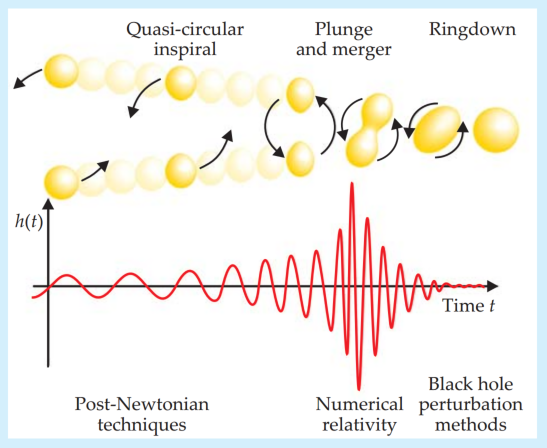
\includegraphics[width=\linewidth]{stages.png}
			\caption{The different stages in the evolution of a BBH system along with the methods used to model each stage. \cite{bbhm} }
			\label{stages}
		\end{figure}
		
	
	Einstein's field equations, being a set of 10 nonlinear coupled partial differential equations, contains thousands of terms when expressed in a general coordinate system. Although linearized weak field approximations to these equations were used by Einstein to predict the existence of gravitational waves in 1916, this method can only be used to study gravitational waves far away from their source of origin. The strong field equations, given some initial conditions, can only be exactly solved analytically for a few simple scenarios which exhibit high symmetry, for example the case of a single isolated static black hole with spin (a Kerr metric). The only possible method to obtain accurate solutions of a dynamical phenomena such as BBH mergers, is to perform numerical simulations. Numerical relativity refers to solving the Einstein's field equations for both the dynamics of matter along with the evolution of the background space-time metric on a computer. This is an extremely complex problem, requiring a tremendous amount of parallel computing resources, which is why numerical relativists were among the first scientists to use supercomputers.
		\newline
	
	 Numerical relativity has a rich history dating back more than half a century \cite{living}. Attempts to solve the problem of binary black hole mergers started in 1964 with Hahn and Lindquist, which were largely unsuccessful due to the lack of computational power at that time. The first successful attempts were made in the 1970s when Smarr and Eppley were able to simulate the head-on collision of two identical black holes with assumptions of axi-symmetry. The first fully 3-D simulations of the head-on collision of two black holes were performed in 1998 by the Grand Challenge Alliance. However, obtaining stable long-term simulations of orbiting BHs proved to be more difficult particularly due to problems with dealing with the singularities of the BHS. It was only in 2005 that the first stable long term evolution of a BBH system, including the merger and ringdown stages, was performed successfully by Pretorius \cite{pret}. Immediately following this, multiple numerical relativity groups were able to develop independent codes using different formulations to completely solve the BBH merger for low mass-ratio systems with zero eccentricities.
		\newline
		
	Despite the fact that numerical relativity has now reached a state of maturity, most of these state-of-the-art codes used today are proprietary (eg. the Spectral Einstein Code developed by the sXs collaboration \cite{sxs} and the code developed by Stuart Shapiro and his group at UIUC). These closed-source codes have been successfully used to exactly reproduce the evolution of the binary black hole system which was the source of GW150914. One of the visualizations created by these codes can be seen in figure \ref{sxs}. However, there are still no freely available open-source codes that can be used by the public to reproduce this observed signal. Therefore, for the sake of promoting transparency in science, it will be worthwhile to release a free and open-source code to do this.
		\newline
	
		\begin{figure}[h]
			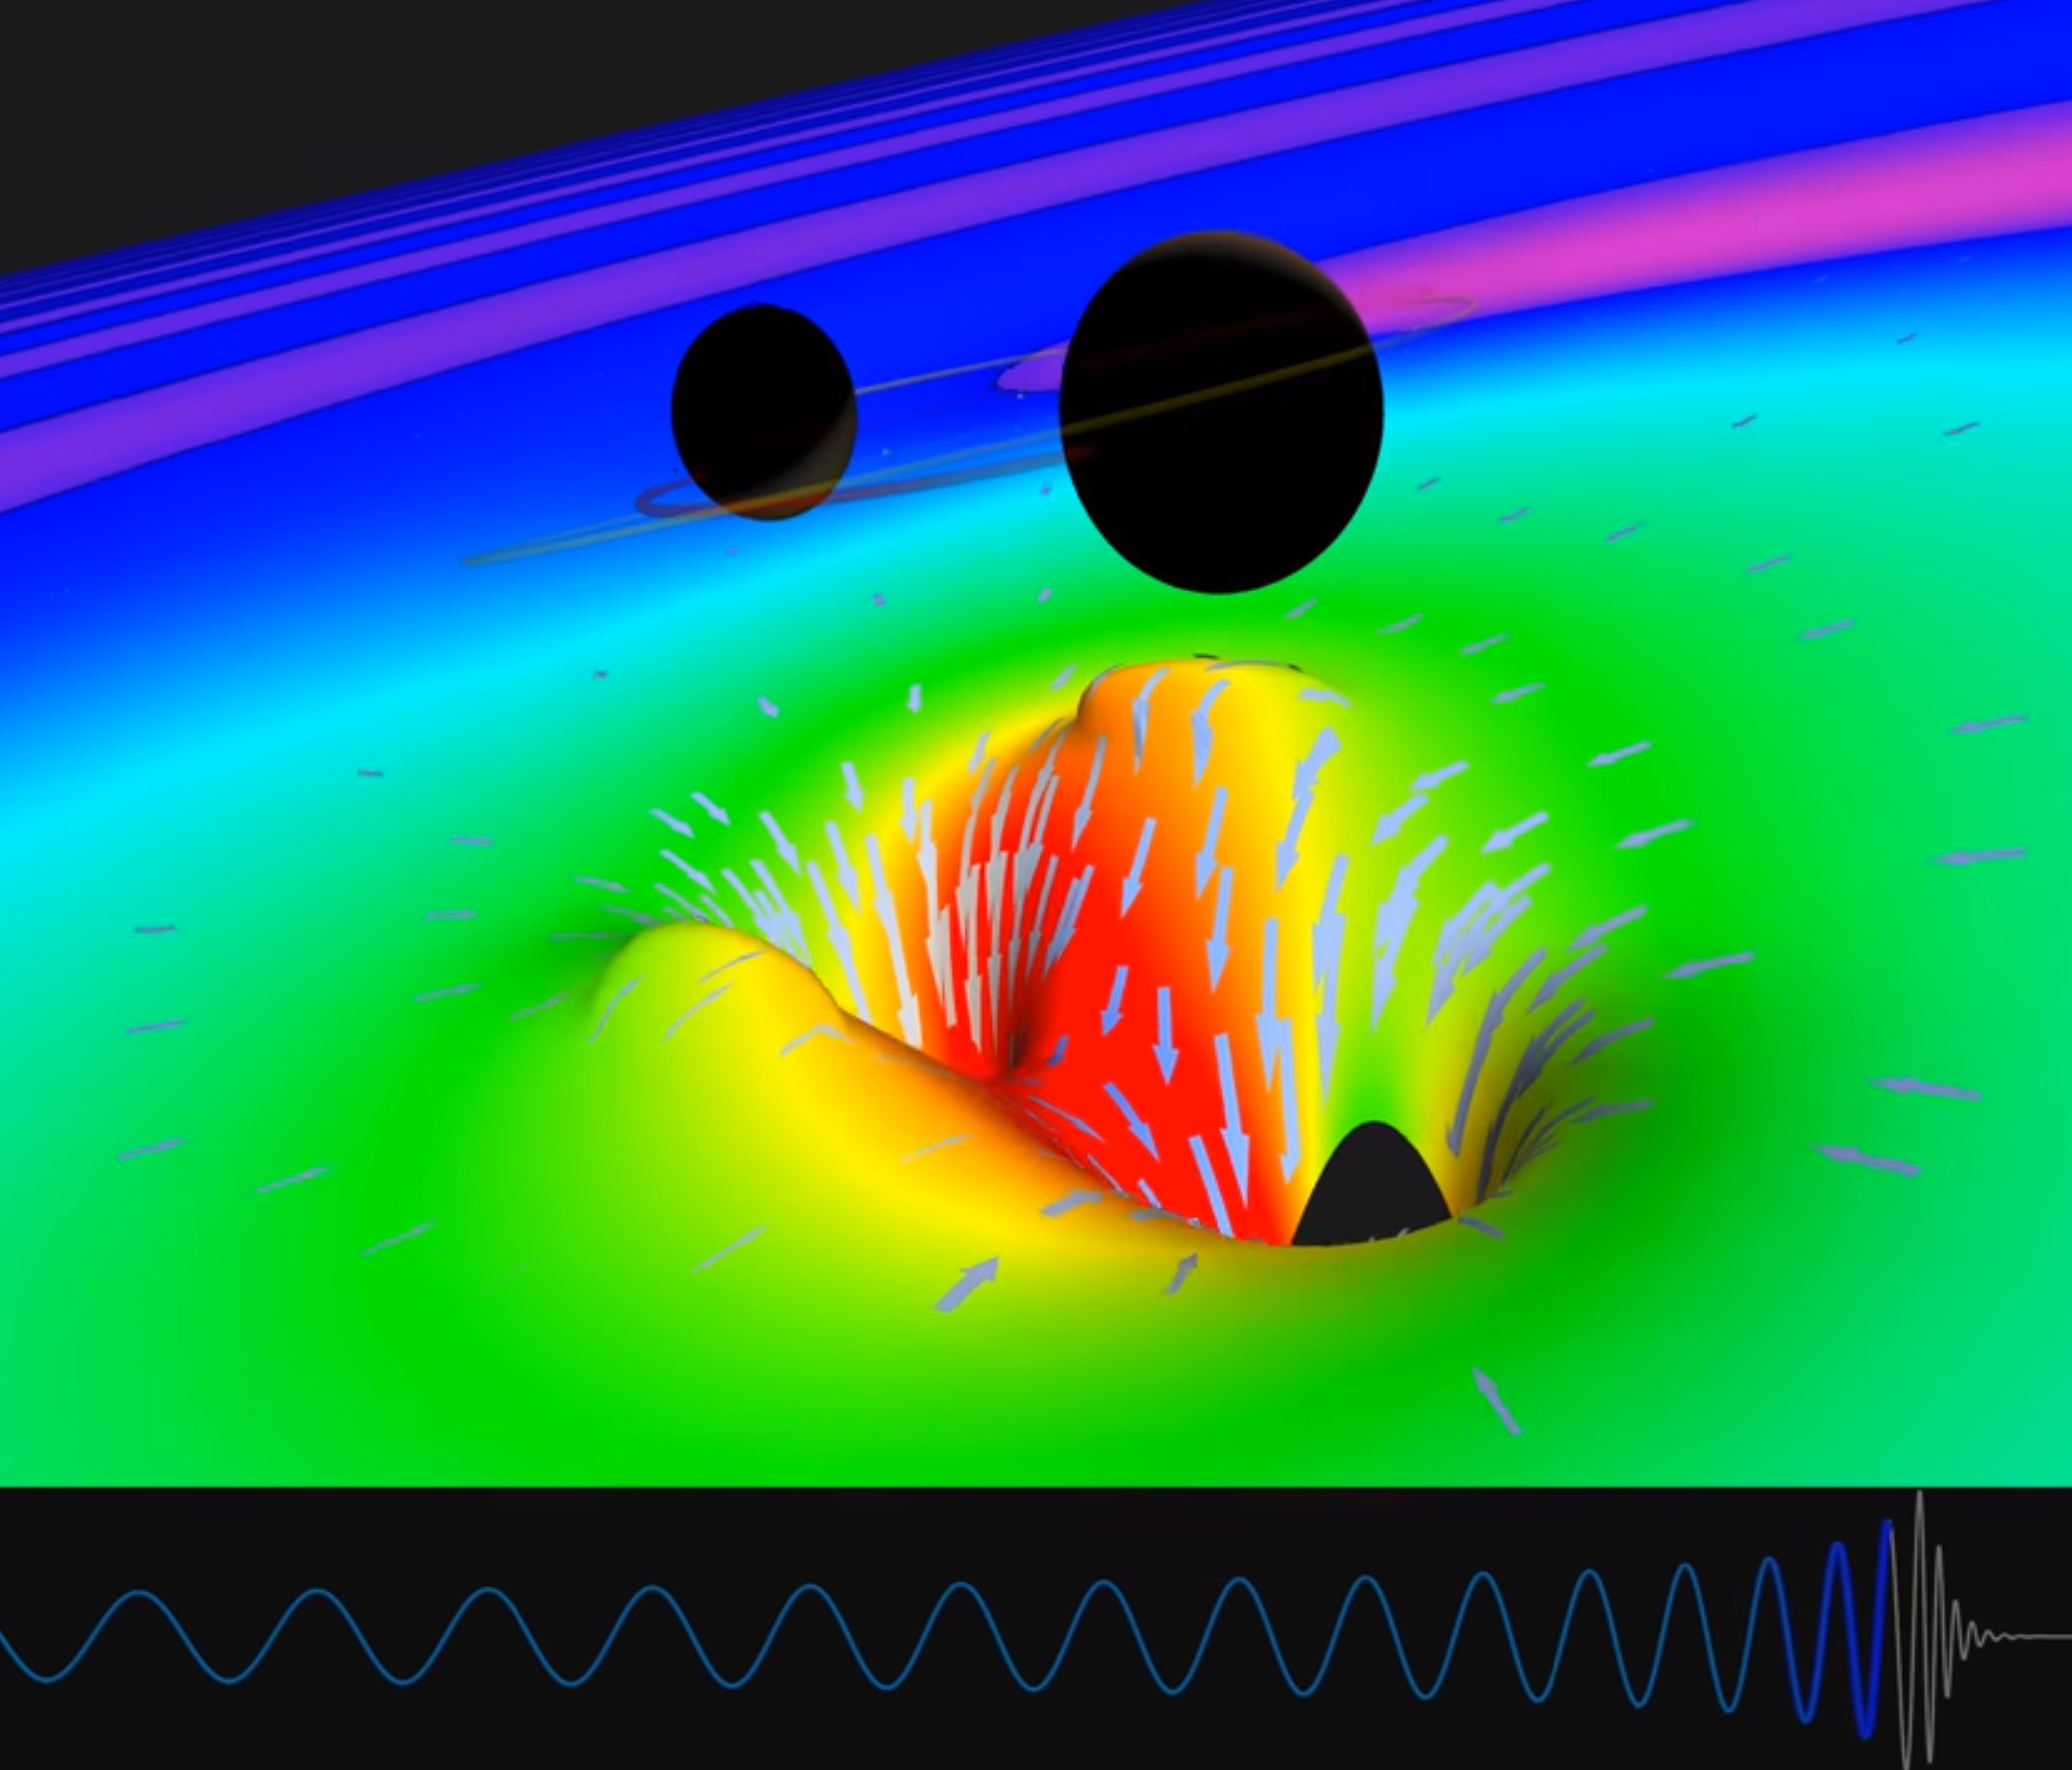
\includegraphics[width=\linewidth]{spec.png}
			\caption{Visualization of GW150914 done by the sXs collaboration with the SPEC code. \cite{sxs}}
			\label{sxs}
		\end{figure}
	
	In the next section, I will give a brief description of the Einstein toolkit and the Cactus framework which it is based upon as well as the equations that are being solved. Following this, I will elaborate on the initial set up of the simulation and the tests done. Then I will present the results including the gravitational waveforms obtained from this simulation. Finally, I will end with a discussion of the importance of these results and the scope for extending the code in the future.
	
	
	
	%%%%%%%%%%%%%%%%%%%%%%%%%%%%%%%%%%%%%%%%%%%%%%%%%%%%%%%%%%%%%%%%%%%%%%%%%%%%%
	\section{Methods}
	 The details of both the software and the numerical schemes that I have used to solve the Einstein's field equations in vacuum space-time for a system of two black holes are discussed in the following subsections.

	\subsection{Software}
	The Cactus framework is an open source modular code originally developed for numerical relativity but later extended to other areas including computational fluid dynamics, cosmology, quantum gravity and has found applications even in the petroleum industry. It is highly portable and can run on diverse architectures from desktops and laptop computers to supercomputers such as Blue Waters. It is based on code developed at the National Center for Supercomputing Applications (NCSA) by Ed Seidel and his group in early 1990s, to solve the BBH merger problem. It was later extensively developed at the Albert Einstein Institute in Germany with version 1.0 released in 1997 \cite{cactus}. Owing to it's open source nature, it quickly gained popularity among multiple numerical relativity groups and has been actively and collaboratively developed since, by contributors from over 20 countries. The vast majority of numerical relativity codes used today are based on Cactus.
		\newline
	
	The Cactus framework consists of a common core or infrastructure, called the Flesh, along with numerous modules	called Thorns, which can be selectively plugged in to implement different functionality. The flesh is only an interface for the thorns and almost every function is handled by various thorns, including memory allocation and MPI parallelization (Driver thorn). Adaptive mesh-refinement is handled by a thorn called Carpet \cite{living}.
		\newline
	
	The Einstein toolkit (ET) is a fork of Cactus, which includes a collection of about 100 public thorns suited specifically for solving problems in numerical relativity \cite{ET}. It is actively maintained by numerical relativists. Simulation factory (SimFactory) is a tool included in the ET, which is used to facilitate running simulations across various supercomputers and clusters with different architectures and queuing systems \cite{intro}. It contains a collaborative database of configurations for each machine, that has been correctly configured at least once by someone using the ET. It also enables amateurs to organize and manage their simulations, while easily adopting the style and conventions used by experienced computational scientists.		
	
	\subsection{Equations}
	The formulation of the equations of general relativity currently used within the Einstein toolkit is known as the 3+1 formalism. Although the original form of Einstein?s equations is deceptively simple and coordinate agnostic, we must choose a proper coordinate system carefully to ensure the stability and convergence of our numerical schemes. We also need to separate out space and time because the initial conditions are specified at a particular point in time.
		\newline
	
	Most numerical relativists today use a modified version of what is known as the Arnowitt-Deser-Misner (ADM) formalism. In the ADM formalism, which was originally developed to study quantum gravity in 1959 \cite{living}, space-time is foliated into space-like 3-dimensional surfaces at different time-like instances (see figure \ref{3+2}). Initial data is specified at a particular 3-D surface. The motion of the bodies are solved at each time step and then the evolution of the metric to the next time step is computed using the equations of the ADM formalism \cite{3+1}. However, it was discovered that the original set of equations used in the ADM formalism were not well-posed, i.e small changes in the initial data led to drastic changes in the solution at a later time. The BSSN (Baumgarte-Shapiro-Shibata-Nakamura) formulation is a modification to the original ADM formalism that transform it into a well-posed set of equations by adding a few auxiliary variables \cite{BS}.
		\newline
		
		\begin{figure}[h]
			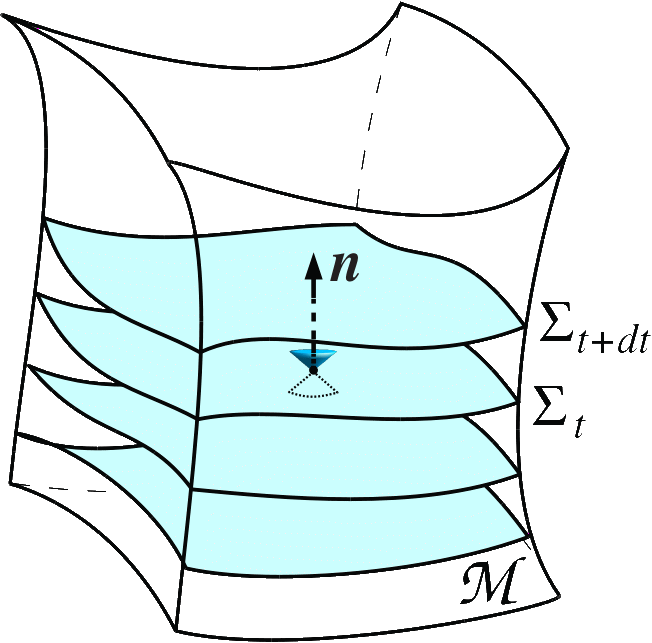
\includegraphics[width=.8\linewidth]{3+1.png}
			\caption{Visualization of the 3+1 formalism; space-time is sliced into space-like surfaces at different coordinate times \cite{3+2}.}
			\label{3+2}
		\end{figure}
	
	
	I am using the McLachlan thorn in the Einstein toolkit, which is a vacuum space time solver generated by KRANC \cite{kranc}, that uses 8th order finite differencing schemes to solve the BSSN formulation of the field equations. KRANC is an open-source Mathematica package that is can generate highly optimized C-code to implement up to 8th order finite-differencing schemes for any system of PDEs in continuous/tensorial form specified in Mathematica syntax \cite{kranc}. The McLachlan thorn contains over a thousand lines of C-code generated by KRANC \cite{intro}.
	
	
	
	\section{Tests and Initial Conditions}
	
	I have tested the Einstein Toolkit using the ``qc0-mclachlan.par'' parameter file that is included with the default installation of ET \cite{intro}. qc0 refers to a simple test of a BBH coalescence commonly used by numerical relativists to check their code. qc0-mclachlan uses the McLachlan thorn as the vacuum space-time solver. All units mentioned in the following sections refer to dimensionless units. The proper dimensions can be restored by inserting factors containing the gravitational constant, speed of light and mass of the sun wherever appropriate. 
	\newline
	
	The initial set up of qc0 consists of two identical, non-spinning, black holes placed at an equal distance from the origin on the x-axis at +/-1.168642873  respectively each with identical momenta pointing along the +/- y-axes with magnitude 0.3. The TwoPunctures thorn is used to generate the initial data for the space-time metric, given the parameters and locations of the BHs. The AHFinder thorn is used to estimate their apparent horizons at each time step. This parameter file specifies reflection symmetry about the z=0 plane as well as a 180$^{\circ}$ rotational symmetry which reduces the total computation time by a factor of 2 each. The Carpet thorn is used for adaptive mesh refinement with 7 levels specified initially and up to 10 levels allowed during the course of the simulation. The simulation domain is a cubical box of side 120 units with isolated boundary conditions. The largest grid size is set to be 64 units.
	\newline
	
	To reproduce GW150914, which was a system of black holes on a quasi-circular orbit with 36 and 29 solar masses, I have modified the ``qc0-mclachlan.par'' file by changing the initial masses to .45 and .36 respectively. The initial guess for the AHFinder thorn was changed to .25 and .2 respectively. The system does not exhibit rotational symmetry since the masses are not identical; therefore I turned off the 180$^{\circ}$ rotational symmetry. The exact linear momenta of these black holes at the given separation are unknown. However, I used Newtonian mechanics to calculate an approximate value of .35 for the linear momentum of each black hole, by assuming perfectly circular orbits for the binary system in flat space-time.
	\newline
	
	I have also performed another simulation by making the same changes to the ``inspiral.par'' included with ET, which calculates the inspiral of two black holes with initial conditions similar to qc0-mclachlan. The results obtained from both simulations are presented in the following section. 
	
	
	
	\section{Results}
	All the simulations were performed on the campus cluster at UIUC using both the original qc0-mclachlan parameter file as well as the modified version of it. The modified version of qc0-mclachlan consumed about 800 CPU hours (twice as much time as the original parameters due to the absence of rotational symmetry). The simulation with the "inspiral.par" file consumed about 400 CPU hours.
	\newline
	
    The information about the gravitational waves are encoded in the Weyl scalar \cite{living}. I have used SimulationTools, an "open-source" Mathematica package by Ian Hinder and Barry Wardell \cite{simtools}, to extract the waveforms from the output of the WeylScalar4 thorn of the Einstein Toolkit. Since the (2,2) mode is the dominant mode for approximately equal mass ratio systems, it is commonly used by numerical relativists to analyze GWs. Furthermore, I have used SimulationTools to extrapolate the Weyl scalar to infinity using the values up to radius 90. Finally, I have computed the strain, which is what the detectors measure physically, by integrating the Weyl scalar using SimulationTools.
    \newline
    
    Plots of waveforms of the Weyl scalar as well as the strain, obtained from the original qc0-mclachlan parameter file alongside the modified parameter file, are shown in figure \ref{weyl} and \ref{strain} respectively.  Plot of the orbits of the center (singularity) of each BH is shown in figure \ref{orbits} up to the merger, after which their individual centers are no longer well defined. SimulationTools was used again to extract the coordinates of the black holes from the hdf5 output of the simulation.
    \newline
    	\begin{figure}[h]
    		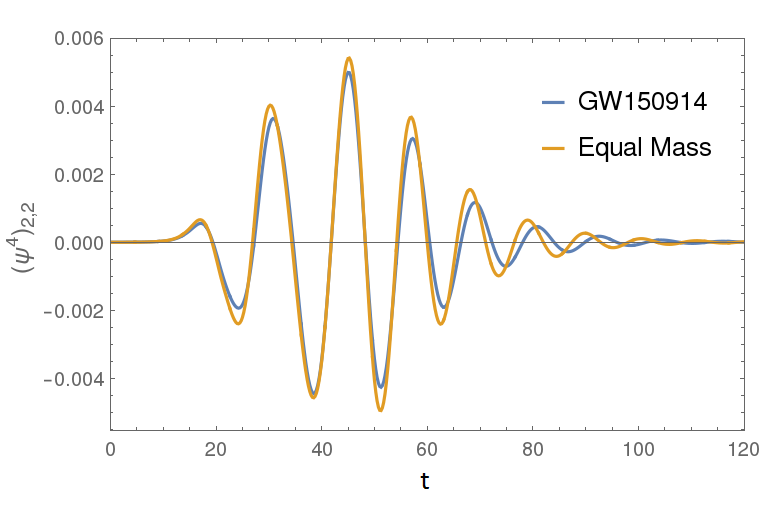
\includegraphics[width=\linewidth]{weyl.png}
    		\caption{Plots of the 2,2 mode of the Weyl scalar ($\psi_{2,2}^{4}$) vs time, extrapolated to infinite distance for both the identical mass system and the GW150914 simulation}
    		\label{weyl}
    	\end{figure}
    		\begin{figure}[h]
    			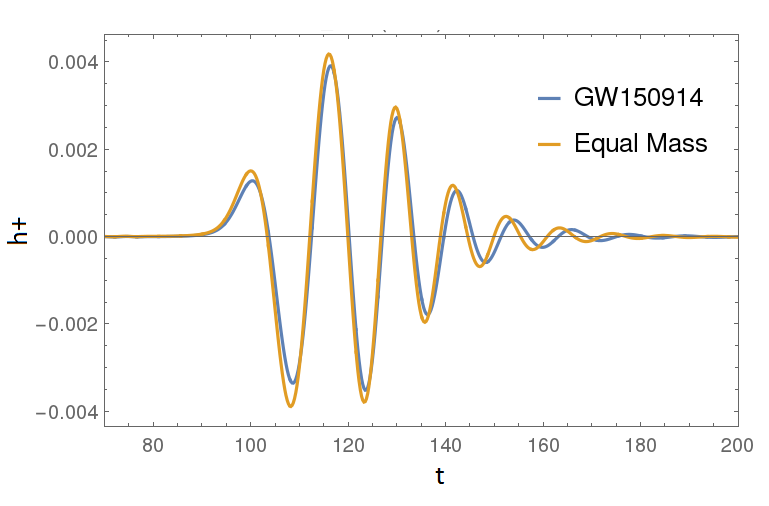
\includegraphics[width=\linewidth]{strain.png}
    			\caption{Plots of the plus component of strain, calculated from ($\psi_{2,2}^{4}$), vs time for both the identical mass system and the GW150914 simulation}
    			\label{strain}
    		\end{figure}
    
   
    	\begin{figure}[h]
    		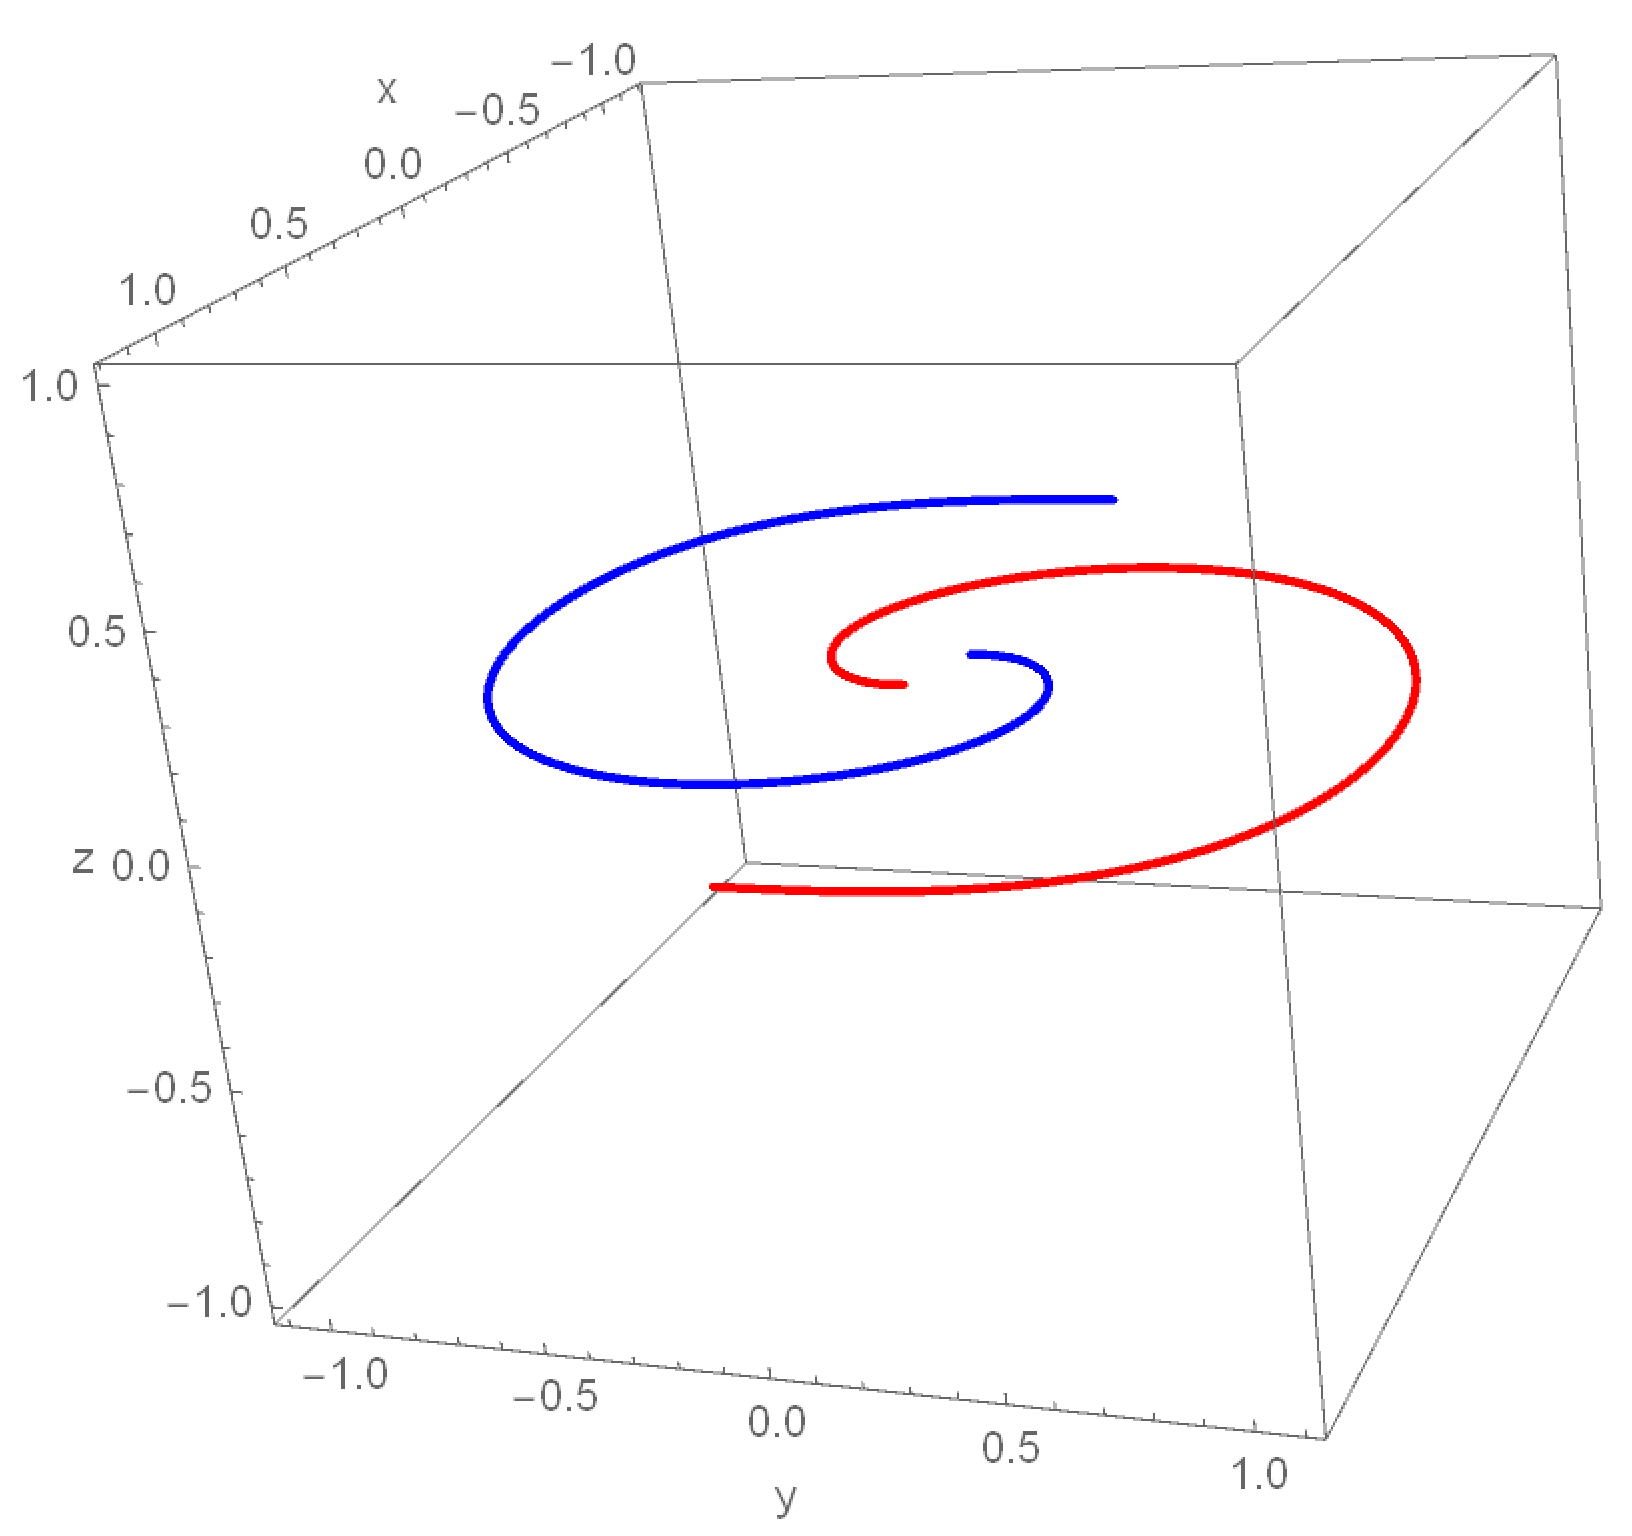
\includegraphics[width=\linewidth]{orbits.png}
    		\caption{Orbits of the BHs from the merger and ringdown simulation}
    		\label{orbits}
    	\end{figure}
  
        The strain computed from the inspiral of the BBH system obtained with the modified "inspiral.par" file is shown in figure \ref{inspiral}.
    	\begin{figure}[h]
    		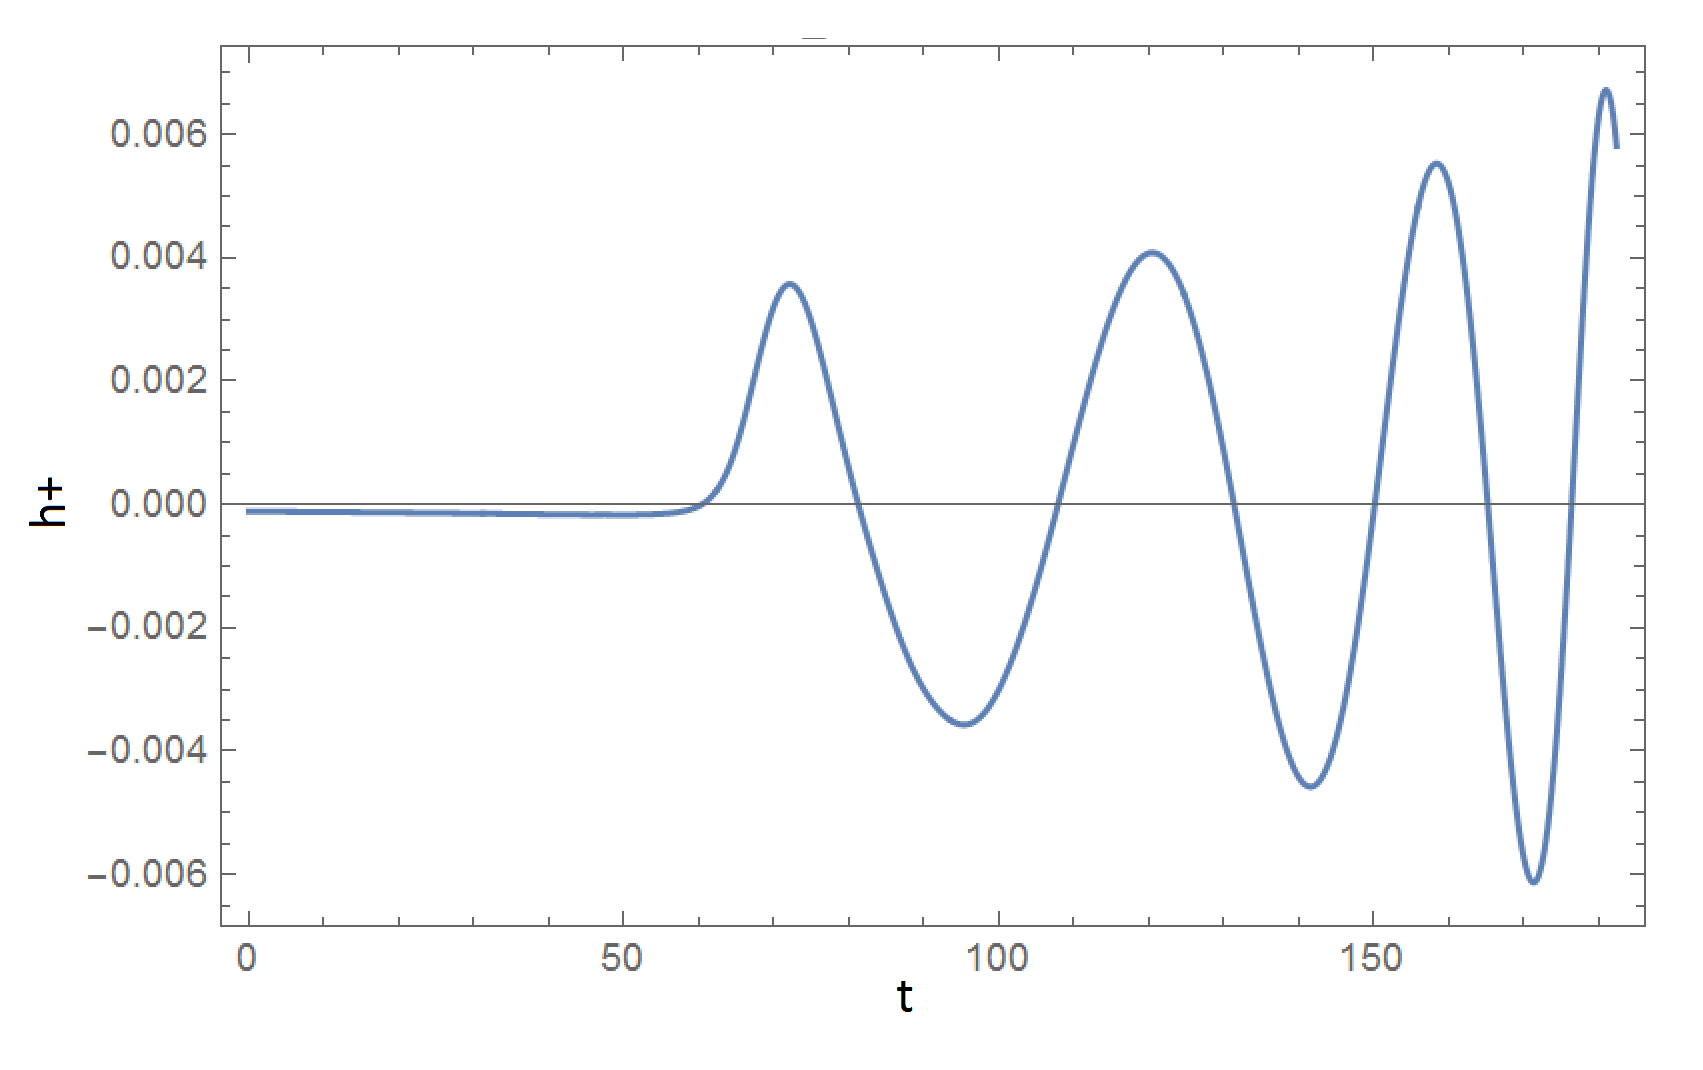
\includegraphics[width=\linewidth]{inspiral.png}
    		\caption{Strain computed from the inspiral simulation.}
    		\label{inspiral}
    	\end{figure}
     

	
	\section{Discussion}
	
	The parameter files used for these simulations can be freely found here: \href{http://tiny.cc/et-gw150914}{http://tiny.cc/et-gw150914}. Instructions for installing and running the Einstein Toolkit can be found at: \href{http://tiny.cc/et-tutorial}{http://tiny.cc/et-tutorial}.
	  \newline
	    
	Since the exact initial momentum is unknown and the simulation starts only from half an orbit before merger, the waveforms I have obtained will not precisely match GW150914. Moreover, even with correct initial momenta, the TwoPuncture thorn which is used to calculate the initial space-time metric is not completely accurate. Therefore the strategy used by most numerical relativists is to start a simulation at the early inspiral phase in order to calculate the space-time at the late inspiral phase, which is then fed as the input to a merger and ringdown simulation. Therefore, I plan to use the output obtained with the modified ``inspiral.par'' file to improve the merger and ringdown waveform.
	\newline
		
	With the ever increasing computational power of supercomputers (soon to enter the exascale regime), we will have the ability to do extremely precise simulations of almost every kind of scenario that we can imagine. However, these simulations are still very	expensive and time-consuming. Therefore, the publicly available catalogs of gravitational waveforms obtained from numerical relativity simulations are very sparse, covering only a small subset of the total parameter space. LIGO currently relies on various semi-analytic models as well as statistical fits in order to quickly generate reasonably accurate waveforms that cover the entire spectrum of possible parameter values. Various free coefficients in these semi-analytic models are obtained through fitting with catalogs of numerical relativity simulations. Thus, increasing the size of the publicly available catalogs by adding more waveforms generated by numerical relativity simulations with the ET, covering a wider range of astrophysical systems would allow us to create and calibrate better semi-analytical and statistical models in the future. Therefore, I intend to install the ET on Blue Waters, and use these parameter files to generate a new catalog of simulations for quasi-circular systems with zero spins for a wide range of mass-ratios.
	  \newline
	  
	Although GW emission is expected to circularize the orbits, the presence of an external perturbation could lead to significant eccentricities in the late inspiral stages. Since catalogs of eccentric systems with or without spins are not available at present, I plan to extend this code to work for systems with high orbital eccentricity. This can then be used to validate or calibrate the semi-analytic code that I recently developed with Eliu Huerta at NCSA, which can generate such waveforms quickly (see figure \ref{ecc} for a sample waveform with non-zero eccentricity).
	\newline
	\begin{figure}[ht]
		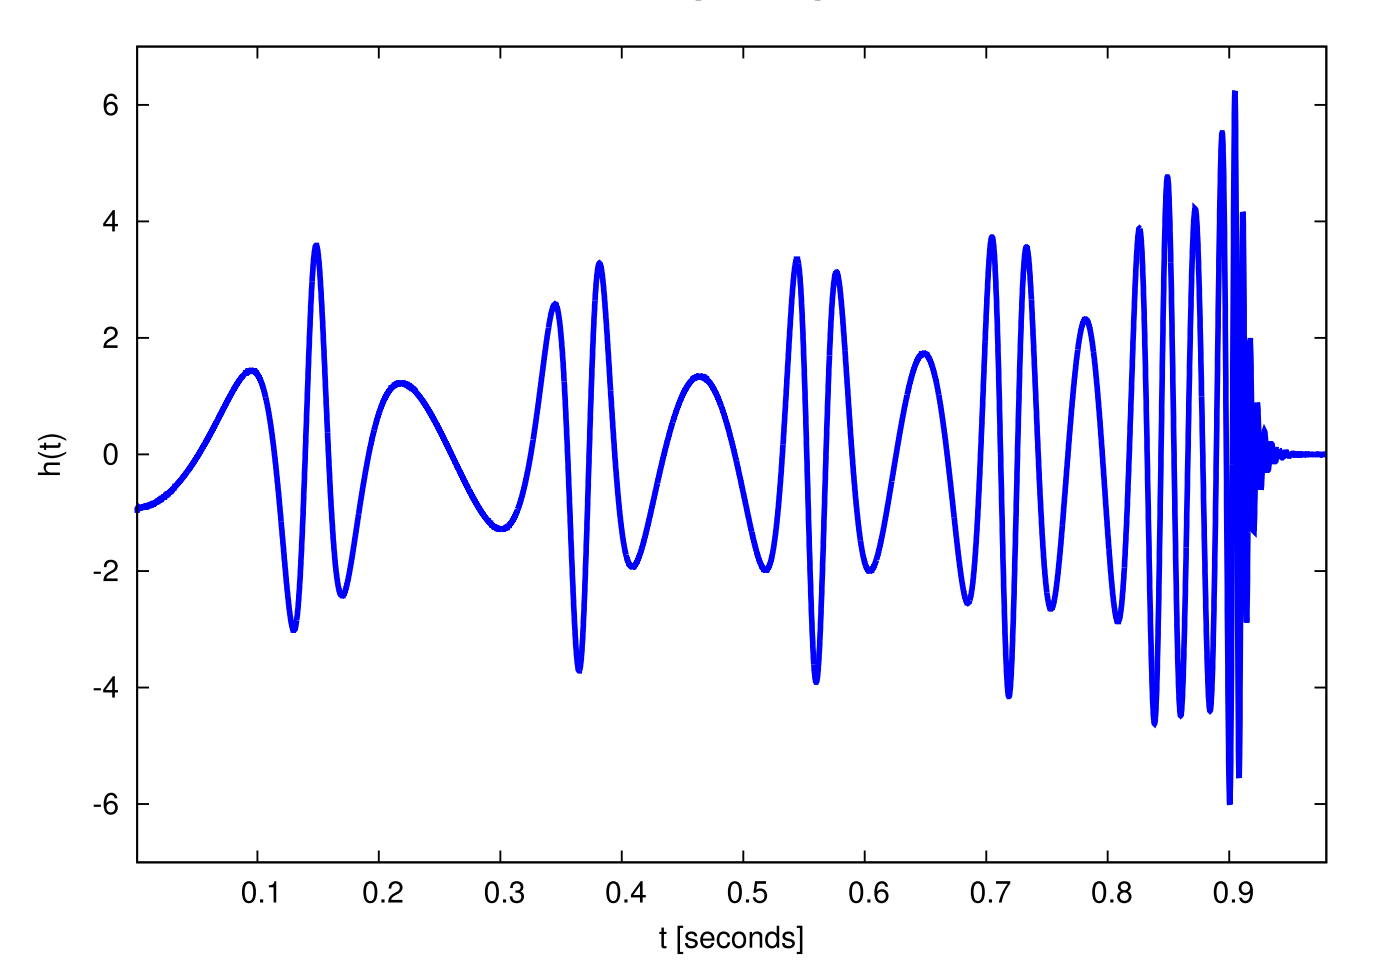
\includegraphics[width=\linewidth]{ecc.png}
		\caption{A sample waveform for a BBH system with 10 solar masses with initial eccentricity = 0.4 at frequency of 10Hz, generated using the semi-analytical model that I developed.}
		\label{ecc}
	\end{figure}
	
	Another possibility is to extend the code to work for systems with high mass-ratios (greater than 1:10), which is a difficult problem, still under active research, due to the large disparity in the scales required for the mesh sizes and refinement levels for each black hole. Furthermore PN methods and gravitational self-force corrections usually fail to model these extreme-mass ratio cases.
	
	
	
	\begin{acknowledgments} I wish to express my deepest gratitude to Dr. Eliu Huerta and Prof. Gabrielle Allen for clarifying my doubts about various aspects of numerical relativity and gravitational wave astronomy. I thank Justin (Hsi-Schive) for his help in getting the Einstein Toolkit up and running perfectly on the campus cluster at UIUC, which was no easy feat. I would also like to thank Roland Haas for his lectures on the Einstein Toolkit and for pointing me towards several tools used for gravitational waveform extraction from simulation data. Most of all, I am forever indebted to Prof. Paul Ricker for his overall guidance on this project along with his invaluable feedback and detailed comments on the numerous drafts of this paper.
		\newpage
	\end{acknowledgments}
	
	\bibliography{sample-paper}
	
	\bibliographystyle{prsty}		
	\begin{thebibliography}{99}
		\bibitem{gw1}
		B. P. Abbott et al., \href{http://journals.aps.org/prl/pdf/10.1103/PhysRevLett.116.061102}{PRL 116, 061102 (2016)}
		\bibitem{nano}
		F. Jenet et al., \href{http://arxiv.org/abs/0909.1058}{arXiv:0909.1058 [astro-ph.IM]} 
		\bibitem{LP}
		 L. Lehner, F. Pretorius, \href{http://arxiv.org/pdf/1405.4840.pdf}{arXiv:1405.4840 [astro-ph.HE]} 
		\bibitem{living}
		  V. Cardoso et al., \href{http://journals.aps.org/prl/abstract/10.1103/PhysRevLett.93.174102}{Living Rev. Relativity 18 (2015), 1} 
		\bibitem{ET} 
		F. Loffler et al., \href{http://arxiv.org/pdf/1111.3344v1.pdf}{	arXiv:1111.3344 [gr-qc]} 
		\bibitem{intro} 
		 M. Zilhao, F. Loffler, \href{http://arxiv.org/abs/1305.5299}{arXiv:1305.5299 [gr-qc]} 
		\bibitem{bbhm}
		T. W. Baumgarte, S. L. Shapiro, \href{http://w.astro.berkeley.edu/~gmarcy/astro160/papers/binary_black_hole_mergers.pdf}{Physics Today, October 2011, page 32} 
		\bibitem{test}
		B. P. Abbott et al., \href{https://arxiv.org/abs/1602.03841}{arXiv:1602.03841 [gr-qc]} 
		\bibitem{quantum}
		 S. B. Giddings, \href{https://arxiv.org/abs/1602.03622}{arXiv:1602.03622 [gr-qc]}
		\bibitem{mimick}
		V. Cardoso, E. Franzin, P. Pani, \href{http://journals.aps.org/prl/abstract/10.1103/PhysRevLett.116.171101}{Phys. Rev. Lett. 116, 171101} 
		 \bibitem{kranc}
		  S. Husa, I. Hinder, C. Lechner, \href{http://arxiv.org/pdf/gr-qc/0404023v2.pdf}{arXiv:gr-qc/0404023} 
		 \bibitem{3+1}
		  M. Alcubierre, \href{http://www.amazon.com/Introduction-Numerical-Relativity-International-Monographs/dp/0199656150}{Introduction to 3+1 Numerical Relativity} 
		 \bibitem{BS}
		  T. W. Baumgarte, S. L. Shapiro, \href{http://www.amazon.com/Numerical-Relativity-Einsteins-Equations-Computer/dp/052151407X}{Numerical Relativity: Solving Einstein's Equations on the Computer} 
		 \bibitem{simtools}
		 I. Hinder, B. Wardell, \href{ http://simulationtools.org/}{http://simulationtools.org/} 
		 
	     \bibitem{pret}
	     F. Pretorius, \href{https://arxiv.org/abs/gr-qc/0507014}{arXiv:gr-qc/0507014}  
		 \bibitem{cactus} 
		 G. Allen et al., \href{http://cactuscode.org/}{http://cactuscode.org/}  
		 \bibitem{3+2} 
		E. Gourgoulhon, \href{https://www.springer.com/us/book/9783642245244}{3+1 Formalism in General Relativity}
		\bibitem{sxs} 
		sXs Collaboration, \href{http://www.black-holes.org/}{http://www.black-holes.org/}
	
	\end{thebibliography}
	%%%%%%%%%%%%%%%%%%%%%%%%%%%%%%%%%%%%%%%%%%%%%%%%%%%%%%%%%%%%%%%%%%%%%%%%%%%%%

	
	
	
	
\end{document}
